% =============================================================================
%  Diplomado en Data Science Aplicada con Python para la Toma de Decisiones
%  Clase 22: Proyecto MNIST --- Imagenes como Datos
%  Arca Continental Ecuador | UDLA
%
%  Compilar: pdflatex -shell-escape presentacion.tex (x2 para refs)
% =============================================================================
\documentclass[aspectratio=169, 11pt]{beamer}

\usepackage[T1]{fontenc}
\usepackage[utf8]{inputenc}
\usepackage[spanish,es-noshorthands]{babel}
\usepackage{FiraSans}
\usepackage{FiraMono}
\renewcommand{\familydefault}{\sfdefault}
\usepackage{graphicx}
\usepackage{tikz}
\usetikzlibrary{arrows.meta, positioning, shapes.geometric, shapes.misc,
  calc, fit, decorations.pathreplacing, backgrounds}
\usepackage{fontawesome5}
\usepackage{minted}
\usepackage{tcolorbox}
\tcbuselibrary{minted, skins, breakable}
\usepackage{booktabs}
\usepackage{colortbl}
\usepackage{multicol}
\usepackage{hyperref}
\usepackage{calc}
\usepackage{amsmath}

\definecolor{arcaRed}{HTML}{C82B40}
\definecolor{arcaDark}{HTML}{6B1525}
\definecolor{udlaCrimson}{HTML}{A31545}
\definecolor{arcaGray}{HTML}{F5F5F5}
\definecolor{arcaLightGray}{HTML}{EBEBEB}
\definecolor{textDark}{HTML}{2D2D2D}
\definecolor{textMuted}{HTML}{6B7280}
\definecolor{codeGreen}{HTML}{16A34A}
\definecolor{codeBlue}{HTML}{2563EB}
\definecolor{codeOrange}{HTML}{EA580C}
\definecolor{codePurple}{HTML}{7C3AED}

\usetheme{default}
\usecolortheme{default}
\setbeamertemplate{navigation symbols}{}
\setbeamertemplate{footline}{}
\setbeamertemplate{headline}{}
\setbeamercolor{normal text}{fg=textDark}
\setbeamercolor{frametitle}{fg=arcaRed, bg=white}
\setbeamercolor{title}{fg=white}
\setbeamercolor{subtitle}{fg=white!85}
\setbeamercolor{author}{fg=white!80}
\setbeamercolor{date}{fg=white!70}
\setbeamercolor{item}{fg=arcaRed}
\setbeamercolor{subitem}{fg=arcaDark}
\setbeamercolor{block title}{fg=white, bg=arcaRed}
\setbeamercolor{block body}{fg=textDark, bg=arcaGray}
\setbeamercolor{block title alerted}{fg=white, bg=codeOrange}
\setbeamercolor{block body alerted}{fg=textDark, bg=arcaGray}
\setbeamercolor{block title example}{fg=white, bg=codeGreen}
\setbeamercolor{block body example}{fg=textDark, bg=arcaGray}
\setbeamercolor{section in toc}{fg=arcaDark}
\setbeamerfont{frametitle}{size=\Large, series=\bfseries}
\setbeamerfont{title}{size=\huge, series=\bfseries}
\setbeamerfont{subtitle}{size=\large}
\setbeamerfont{author}{size=\normalsize}
\setbeamerfont{date}{size=\small}
\setbeamerfont{block title}{size=\normalsize, series=\bfseries}
\setbeamerfont{footnote}{size=\tiny}
\setbeamertemplate{itemize item}{\scriptsize\raise1.5pt\hbox{\color{arcaRed}$\blacktriangleright$}}
\setbeamertemplate{itemize subitem}{\scriptsize\raise1pt\hbox{\color{arcaDark}$\bullet$}}
\setbeamertemplate{enumerate items}[default]
\setbeamercolor{enumerate item}{fg=arcaRed}

\setbeamertemplate{headline}{%
  \begin{tikzpicture}[remember picture, overlay]
    \fill[arcaDark] (current page.north west) rectangle
      ([yshift=-0.7cm]current page.north east);
    \node[anchor=west, inner sep=0pt] at
      ([xshift=0.6cm, yshift=-0.35cm]current page.north west)
      {
\includegraphics[height=0.45cm]{../logo_udla_white.png}};
    \node[anchor=east, inner sep=0pt] at
      ([xshift=-0.6cm, yshift=-0.35cm]current page.north east)
      {
\includegraphics[height=0.45cm]{../ArcaContinental_white.png}};
  \end{tikzpicture}%
  \vspace{0.7cm}%
}

\setbeamertemplate{footline}{%
  \begin{tikzpicture}[remember picture, overlay]
    \node[anchor=south east, font=\scriptsize\bfseries\color{arcaRed}] at
      ([xshift=-0.5cm, yshift=0.15cm]current page.south east)
      {\insertframenumber};
  \end{tikzpicture}%
  \vspace{0.3cm}%
}

\setbeamertemplate{frametitle}{%
  \vspace{0.25cm}%
  \usebeamerfont{frametitle}\usebeamercolor[fg]{frametitle}\insertframetitle%
  \par\vspace{2pt}%
  \begin{tikzpicture}
    \fill[arcaRed] (0,0) rectangle (3cm, 1.5pt);
    \fill[arcaLightGray] (3cm,0) rectangle (\textwidth, 0.5pt);
  \end{tikzpicture}%
  \vspace{0.1cm}%
}

\newtcblisting{pyblock}[1][]{%
  listing engine=minted, minted language=python, minted style=friendly,
  minted options={fontsize=\small, linenos=false, breaklines=true, python3=true},
  colback=arcaGray, colframe=arcaRed, left=4pt, right=4pt, top=4pt, bottom=4pt,
  boxrule=0pt, leftrule=3pt, arc=2pt, listing only, #1}

\newtcblisting{outputblock}[1][]{%
  listing engine=minted, minted language=text, minted style=bw,
  minted options={fontsize=\small, breaklines=true},
  colback=white, colframe=arcaLightGray, left=4pt, right=4pt, top=4pt, bottom=4pt,
  boxrule=0.5pt, arc=2pt, listing only,
  title={\small\faTerminal\hspace{6pt}Output}, coltitle=textMuted,
  fonttitle=\small\ttfamily, colbacktitle=white, #1}

\newcommand{\sectionframe}[2]{%
  \begingroup
  \setbeamertemplate{headline}{}%
  \setbeamertemplate{footline}{}%
  \begin{frame}[plain, noframenumbering]
    \begin{tikzpicture}[remember picture, overlay]
      \fill[arcaRed] (current page.south west) rectangle (current page.north east);
      \node[anchor=center, text=white, font=\Huge\bfseries, text width=12cm,
            align=center] at ([yshift=0.5cm]current page.center) {#1};
      \node[anchor=center, text=white!80, font=\large, text width=10cm,
            align=center] at ([yshift=-0.8cm]current page.center) {#2};
    \end{tikzpicture}
  \end{frame}
  \endgroup
}

\title{Diplomado en Data Science Aplicada\\con Python para la Toma de Decisiones}
\subtitle{Clase 22: Proyecto MNIST --- Im\'agenes como Datos}
\author{Carlos Enrique Mosquera Trujillo}
\date{11 de Mayo, 2026}

\begin{document}

% ── PORTADA ──────────────────────────────────────────────────────────────────
{
\setbeamertemplate{headline}{}
\setbeamertemplate{footline}{}
\begin{frame}[plain, noframenumbering]
  \begin{tikzpicture}[remember picture, overlay]
    \fill[arcaDark] (current page.south west) rectangle (current page.north east);
    \fill[arcaRed] ([yshift=-3.5cm]current page.north west) rectangle
      ([yshift=-4.2cm]current page.north east);
    \node[anchor=west, inner sep=0pt] at
      ([xshift=1cm, yshift=-1.5cm]current page.north west)
      {
\includegraphics[height=1cm]{../logo_udla_white.png}};
    \node[anchor=east, inner sep=0pt] at
      ([xshift=-1cm, yshift=-1.5cm]current page.north east)
      {
\includegraphics[height=1cm]{../ArcaContinental_white.png}};
  \end{tikzpicture}
  \vspace{2.5cm}
  \begin{center}
    {\usebeamerfont{title}\usebeamercolor[fg]{title}\inserttitle\par}
    \vspace{0.4cm}
    {\usebeamerfont{subtitle}\usebeamercolor[fg]{subtitle}\insertsubtitle\par}
    \vspace{0.6cm}
    {\usebeamerfont{author}\usebeamercolor[fg]{author}\insertauthor\par}
    \vspace{0.15cm}
    {\usebeamerfont{date}\usebeamercolor[fg]{date}\insertdate\par}
  \end{center}
\end{frame}
}

% ── MÓDULO 4 ─────────────────────────────────────────────────────────────────
{
\setbeamertemplate{headline}{}
\setbeamertemplate{footline}{}
\begin{frame}[plain, noframenumbering]
  \begin{tikzpicture}[remember picture, overlay]
    \fill[arcaDark] (current page.south west) rectangle (current page.north east);
    \node[anchor=center, text=white, font=\Large\bfseries, text width=12cm,
          align=center] at ([yshift=1cm]current page.center)
      {M\'odulo 4 --- Proyecto};
    \node[anchor=center, text=white!90, font=\huge\bfseries, text width=12cm,
          align=center] at ([yshift=-0.3cm]current page.center)
      {Machine Learning con Im\'agenes};
  \end{tikzpicture}
\end{frame}
}

% ── ROADMAP ─────────────────────────────────────────────────────────────────
\begin{frame}[shrink=22]{Hoja de Ruta de Hoy}
  \vspace{-4pt}
  \begin{center}
  \begin{tikzpicture}[
    node distance=0.35cm,
    roadstep/.style={rectangle, rounded corners=4pt, draw=arcaRed, fill=arcaRed!8,
                 minimum width=11cm, minimum height=0.65cm,
                 font=\footnotesize\bfseries\color{arcaDark}, align=left,
                 text width=10cm, inner sep=6pt},
    num/.style={circle, fill=arcaRed, text=white, font=\scriptsize\bfseries,
                minimum size=0.5cm, inner sep=0pt},
  ]
    \node[roadstep] (s0) {\hspace{0.8cm}MNIST: historia y por qu\'e importa};
    \node[roadstep, below=of s0] (s1) {\hspace{0.8cm}Im\'agenes como datos: cargar, entender, aplanar};
    \node[roadstep, below=of s1] (s2) {\hspace{0.8cm}EDA de im\'agenes: promedios, varianza, distribuciones};
    \node[roadstep, below=of s2] (s3) {\hspace{0.8cm}Preprocesamiento: normalizar pixeles};
    \node[roadstep, below=of s3] (s4) {\hspace{0.8cm}Modelos: log\'istica y RF + confusion matrix + an\'alisis de errores};
    \node[roadstep, below=of s4] (s5) {\hspace{0.8cm}Gradio: dibujar un d\'igito y que el modelo lo prediga};
    \node[roadstep, below=of s5] (s6) {\hspace{0.8cm}Fashion MNIST: el techo de nuestras herramientas};
    \node[roadstep, below=of s6] (s7) {\hspace{0.8cm}?`Qu\'e sigue? Una ventana a redes neuronales};

    \node[num] at ([xshift=0.45cm]s0.west) {1};
    \node[num] at ([xshift=0.45cm]s1.west) {2};
    \node[num] at ([xshift=0.45cm]s2.west) {3};
    \node[num] at ([xshift=0.45cm]s3.west) {4};
    \node[num] at ([xshift=0.45cm]s4.west) {5};
    \node[num] at ([xshift=0.45cm]s5.west) {6};
    \node[num] at ([xshift=0.45cm]s6.west) {7};
    \node[num] at ([xshift=0.45cm]s7.west) {8};
  \end{tikzpicture}
  \end{center}
\end{frame}

% =============================================================================
%  BLOQUE A: MNIST HISTORIA
% =============================================================================
\sectionframe{MNIST}{El ``Hello World'' del Machine Learning}

\begin{frame}{La Historia de MNIST}
  \vspace{-4pt}
  {\footnotesize\color{arcaDark}\bfseries
    MNIST es el dataset m\'as famoso de la historia del ML.
    Todo comenz\'o con un problema real: leer cheques bancarios.}

  \vspace{6pt}
  {\footnotesize
  \begin{itemize}\setlength{\itemsep}{4pt}
    \item[{\color{arcaRed}\scriptsize\faArrowRight}]
      \textbf{1980s:} el servicio postal de EE.UU. necesitaba leer
      c\'odigos postales escritos a mano. Millones de cartas al d\'ia.
    \item[{\color{arcaRed}\scriptsize\faArrowRight}]
      \textbf{1994:} NIST (National Institute of Standards and Technology)
      crea una base de datos de d\'igitos escritos por empleados del censo.
    \item[{\color{arcaRed}\scriptsize\faArrowRight}]
      \textbf{1998:} Yann LeCun (hoy director de IA en Meta) publica
      el paper ``Gradient-Based Learning Applied to Document Recognition''.
      Crea el \textbf{Modified NIST (MNIST)}: 70\,000 im\'agenes de
      28$\times$28 pixeles.
    \item[{\color{codeGreen}\scriptsize\faArrowRight}]
      \textbf{Hoy:} MNIST es el primer dataset que todo estudiante de ML
      usa. Es tan fundamental como ``Hello World'' en programaci\'on.
  \end{itemize}
  }
\end{frame}

\begin{frame}{?`Qu\'e Hay en MNIST?}
  \vspace{-4pt}
  {\scriptsize
  \begin{tabular}{@{}llp{7cm}@{}}
    \toprule
    \textbf{Propiedad} & \textbf{Valor} & \textbf{Detalle} \\
    \midrule
    Im\'agenes & 70\,000 & 60K train + 10K test. Nosotros usaremos 15K (subset). \\
    Tama\~no & 28 $\times$ 28 & Cada imagen son 784 pixeles (= 784 variables). \\
    Pixeles & 0--255 & 0 = negro, 255 = blanco. Escala de grises. \\
    Clases & 10 & D\'igitos 0, 1, 2, \ldots, 9. \\
    Balance & Aprox. 10\% cada & No hay desbalance significativo. \\
    \bottomrule
  \end{tabular}
  }

  \vspace{6pt}
  \begin{tcolorbox}[colback=arcaGray, colframe=arcaRed, boxrule=0.5pt, arc=2pt,
    left=6pt, right=6pt, top=4pt, bottom=4pt]
    {\scriptsize\color{arcaDark}
    \faKey\hspace{4pt}\textbf{Hoy vamos a aplicar TODO lo que sabemos}
    (EDA, preprocesamiento, log\'istica, Random Forest, confusion matrix,
    an\'alisis de errores, Gradio) a este dataset de im\'agenes.
    Mismas herramientas, datos completamente distintos.}
  \end{tcolorbox}
\end{frame}

\begin{frame}[shrink=18]{As\'i Se Ven los D\'igitos}
  \vspace{-4pt}
  \begin{center}
    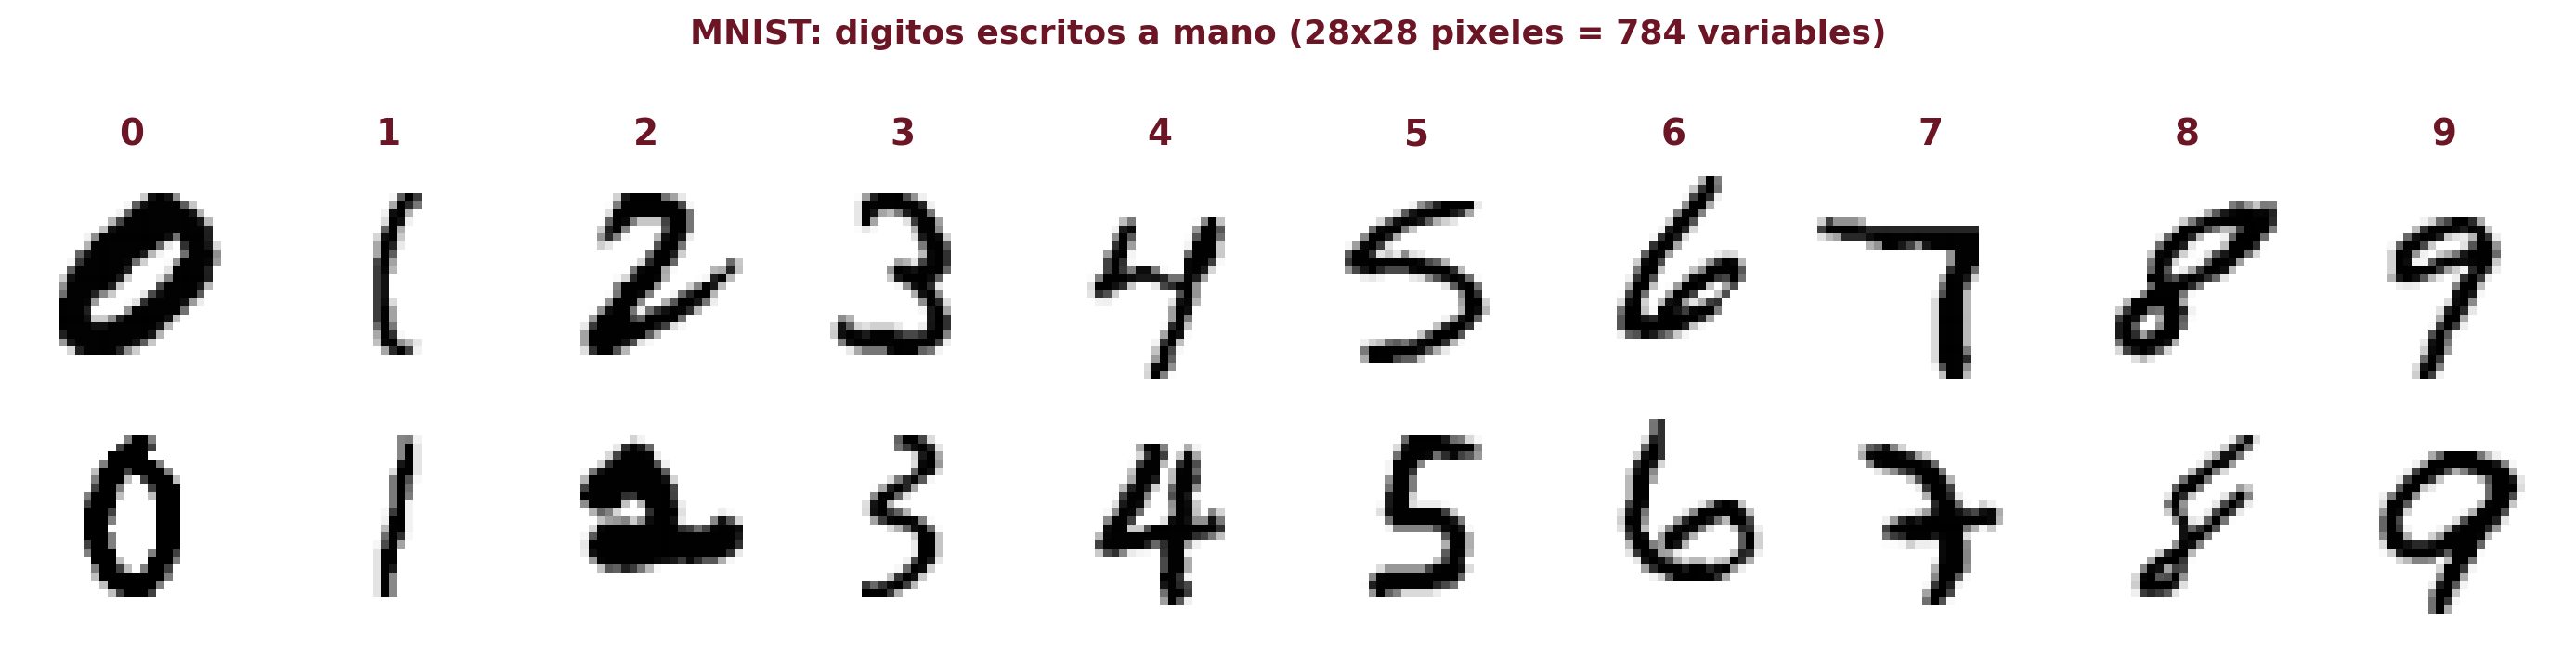
\includegraphics[width=0.9\textwidth]{fig_mnist_samples.png}
  \end{center}

  \vspace{-2pt}
  {\scriptsize\color{textMuted}
    \faLightbulb\hspace{4pt} Cada persona escribe distinto. Un ``7'' puede
    tener barra o no. Un ``1'' puede ser vertical o inclinado. El modelo
    tiene que aprender a reconocer el d\'igito a pesar de la variabilidad.}
\end{frame}

% =============================================================================
%  BLOQUE B: IM\'AGENES COMO DATOS
% =============================================================================
\sectionframe{Im\'agenes como Datos}{De pixeles a DataFrame}

\begin{frame}{Una Imagen Es una Matriz de N\'umeros}
  \vspace{-4pt}
  {\footnotesize\color{arcaDark}\bfseries
    Para la computadora, una imagen no es una ``foto''.
    Es una \textbf{matriz de n\'umeros}:}

  \vspace{6pt}
  {\footnotesize
  \begin{itemize}\setlength{\itemsep}{5pt}
    \item[{\color{arcaRed}\scriptsize\faArrowRight}]
      \textbf{Escala de grises:} una matriz 2D (alto $\times$ ancho).
      Cada celda es un pixel con intensidad 0 (negro) a 255 (blanco).
    \item[{\color{arcaRed}\scriptsize\faArrowRight}]
      \textbf{Color (RGB):} tres matrices 2D apiladas --- una para
      Rojo, una para Verde, una para Azul. Cada pixel tiene 3 valores.
    \item[{\color{codeGreen}\scriptsize\faArrowRight}]
      MNIST es escala de grises: $28 \times 28 = 784$ n\'umeros por imagen.
  \end{itemize}
  }

  \vspace{4pt}
  {\scriptsize
  \begin{tabular}{@{}lll@{}}
    \toprule
    \textbf{Tipo} & \textbf{Imagen 28$\times$28} & \textbf{Imagen 100$\times$100} \\
    \midrule
    Grises & 784 valores & 10\,000 valores \\
    RGB & 2\,352 valores & 30\,000 valores \\
    \bottomrule
  \end{tabular}
  }

  \vspace{4pt}
  {\scriptsize\color{textMuted}
    \faLightbulb\hspace{4pt} Para usar una imagen en ML, la \textbf{aplanamos}:
    la matriz de 28$\times$28 se convierte en un \textbf{vector de 784 n\'umeros}
    --- una fila del DataFrame.}
\end{frame}

\begin{frame}[fragile,shrink=18]{C\'odigo: Cargar MNIST}
  \vspace{-6pt}
  \begin{pyblock}
from sklearn.datasets import fetch_openml
import numpy as np

X, y = fetch_openml("mnist_784", version=1,
                     return_X_y=True, as_frame=False, parser="auto")

# Subset de 15K para velocidad
rng = np.random.default_rng(42)
idx = rng.choice(len(X), 15000, replace=False)
X, y = X[idx], y[idx]

print(f"Imagenes: {X.shape[0]}")      # 15000
print(f"Pixeles:  {X.shape[1]}")      # 784
print(f"Rango:    {X.min()}-{X.max()}")  # 0-255
print(f"Una imagen: {X[0].reshape(28,28).shape}")
  \end{pyblock}

  \vspace{4pt}
  {\scriptsize\color{arcaDark}
    \faKey\hspace{4pt} Cada fila de \texttt{X} son 784 n\'umeros ---
    los valores de intensidad de cada pixel, aplanados.
    Para ver la imagen: \texttt{X[0].reshape(28, 28)}.}
\end{frame}

% =============================================================================
%  BLOQUE C: EDA DE IM\'AGENES
% =============================================================================
\sectionframe{EDA de Im\'agenes}{Explorar datos que no son tablas}

\begin{frame}{EDA de Im\'agenes: ?`Qu\'e Preguntas Hacer?}
  \vspace{-4pt}
  {\footnotesize\color{arcaDark}\bfseries
    No podemos hacer \texttt{df.describe()} en im\'agenes.
    Las preguntas son distintas:}

  \vspace{6pt}
  {\footnotesize
  \begin{enumerate}\setlength{\itemsep}{4pt}
    \item[{\color{arcaRed}\bfseries 1.}]
      ?`C\'omo se \textbf{distribuyen las clases}? ?`Hay desbalance?
    \item[{\color{arcaRed}\bfseries 2.}]
      ?`C\'omo se ve el \textbf{d\'igito promedio} de cada clase?
      ?`Qu\'e pixeles se activan siempre?
    \item[{\color{arcaRed}\bfseries 3.}]
      ?`Qu\'e pixeles tienen m\'as \textbf{varianza}? (Los que var\'ian
      mucho entre im\'agenes son los informativos.)
    \item[{\color{arcaRed}\bfseries 4.}]
      ?`Qu\'e pixeles est\'an siempre en cero? (Las esquinas --- son
      in\'utiles, no aportan informaci\'on.)
    \item[{\color{arcaRed}\bfseries 5.}]
      ?`Hay im\'agenes \textbf{dif\'iciles}? (D\'igitos mal escritos,
      ambiguos, que un humano tambi\'en confundir\'ia.)
  \end{enumerate}
  }
\end{frame}

\begin{frame}[shrink=18]{El D\'igito Promedio: Qu\'e Pixeles Se Activan}
  \vspace{-4pt}
  \begin{center}
    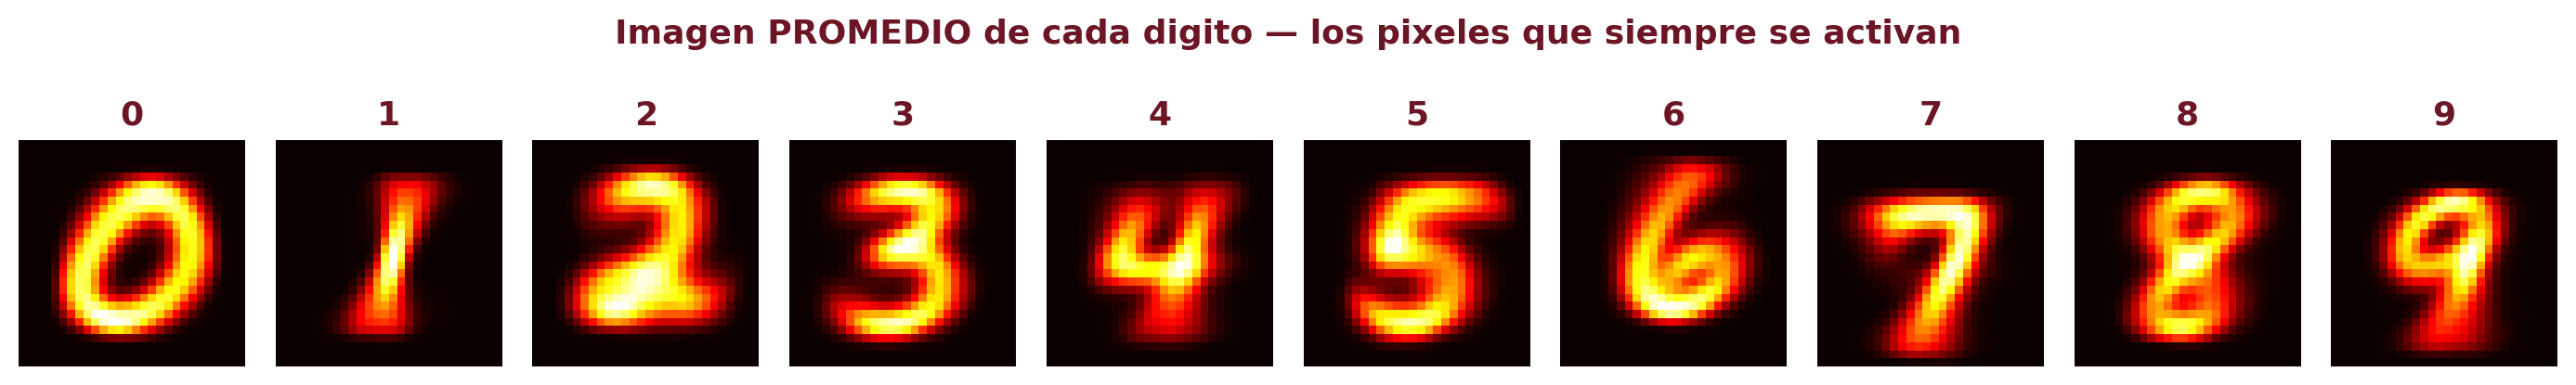
\includegraphics[width=0.9\textwidth]{fig_mnist_promedios.png}
  \end{center}

  \vspace{-2pt}
  {\scriptsize\color{textMuted}
    \faLightbulb\hspace{4pt} El promedio de todos los ``3'' muestra
    qu\'e pixeles se activan \textbf{siempre} cuando alguien escribe un 3.
    El ``0'' activa un anillo, el ``1'' una l\'inea vertical.
    Estos patrones son lo que el modelo aprende.}
\end{frame}

\begin{frame}[shrink=18]{Varianza por Pixel: D\'onde Est\'a la Informaci\'on}
  \vspace{-4pt}
  \begin{center}
    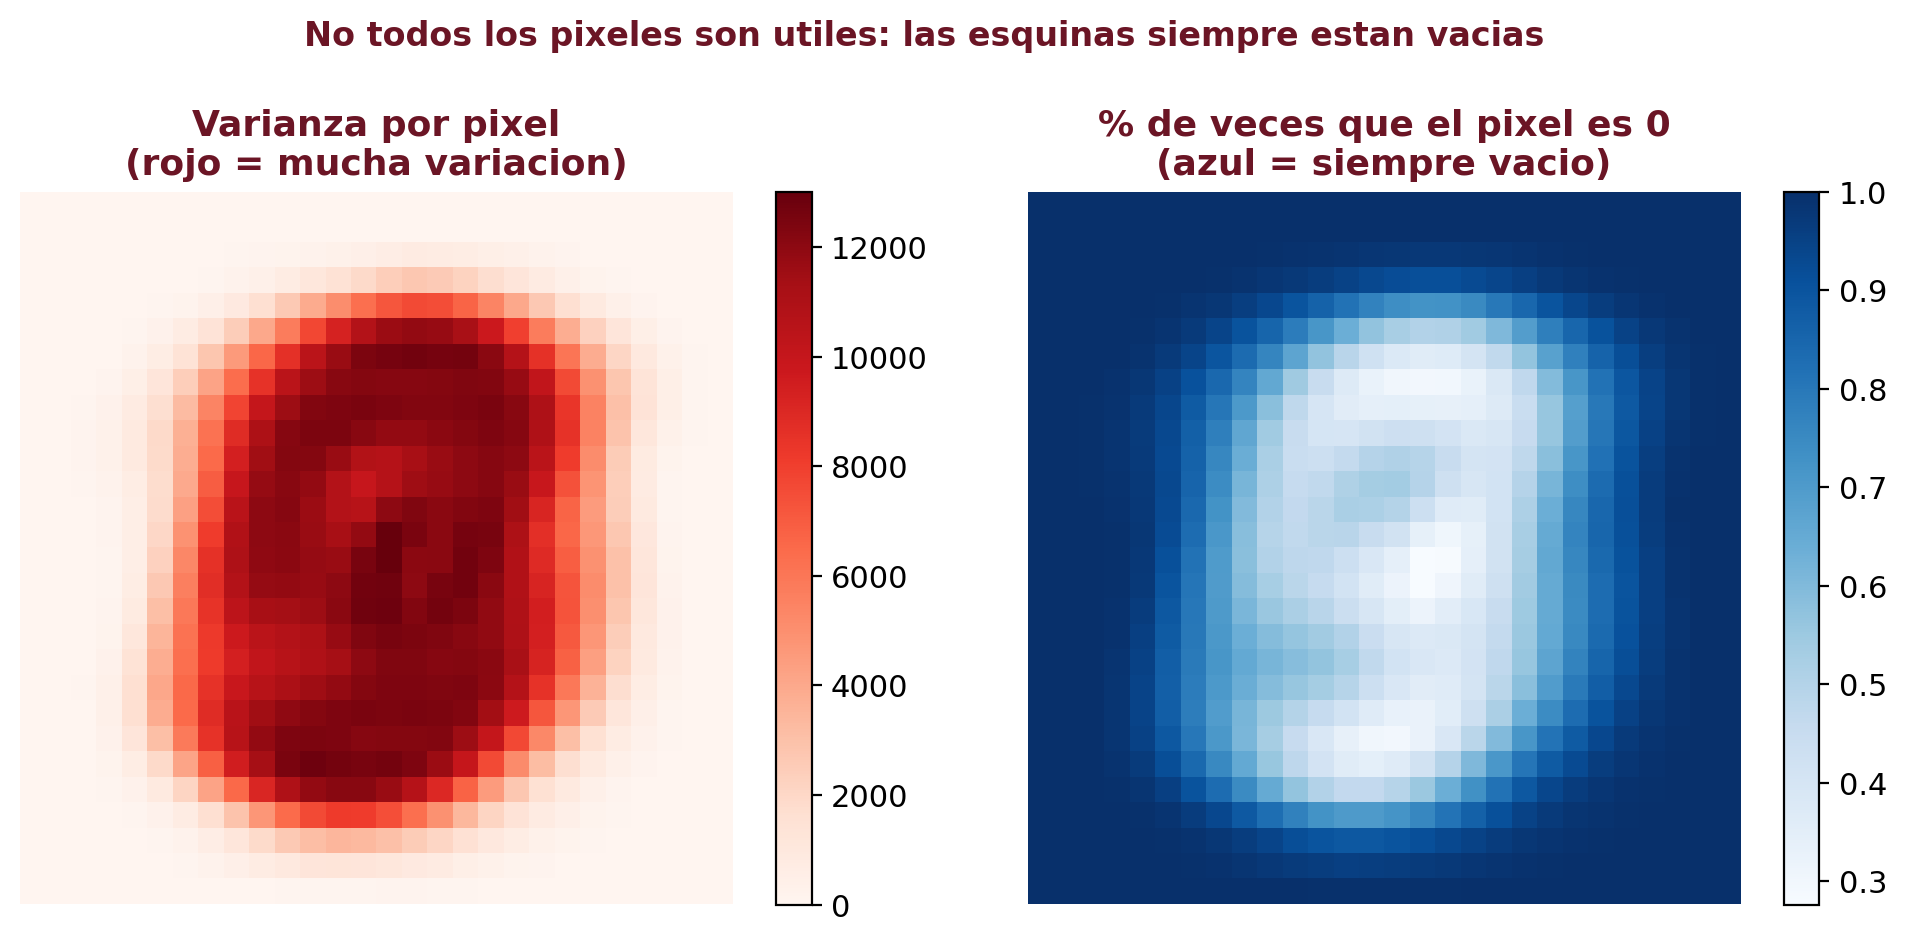
\includegraphics[width=0.78\textwidth]{fig_mnist_varianza.png}
  \end{center}

  \vspace{-2pt}
  {\scriptsize\color{textMuted}
    \faLightbulb\hspace{4pt} \textbf{Izquierda:} los pixeles del centro
    var\'ian mucho (rojo) --- es donde se escriben los d\'igitos.
    \textbf{Derecha:} las esquinas siempre est\'an vac\'ias (azul oscuro).
    De 784 pixeles, muchos son \textbf{in\'utiles}. El modelo tiene que
    encontrar los informativos entre el ruido.}
\end{frame}

% =============================================================================
%  BLOQUE D: PREPROCESAMIENTO
% =============================================================================
\sectionframe{Preprocesamiento}{Preparar las im\'agenes para el modelo}

\begin{frame}[fragile,shrink=10]{Normalizar: Dividir entre 255}
  \vspace{-4pt}
  {\footnotesize\color{arcaDark}\bfseries
    Los pixeles van de 0 a 255. Los modelos lineales funcionan mejor
    con valores entre 0 y 1:}

  \vspace{4pt}
  \begin{pyblock}
# Normalizar: de [0, 255] a [0, 1]
X_train_n = X_train / 255.0
X_test_n  = X_test / 255.0

print(f"Antes: {X_train.min()}-{X_train.max()}")
print(f"Despues: {X_train_n.min():.1f}-{X_train_n.max():.1f}")
  \end{pyblock}

  \vspace{4pt}
  {\scriptsize\color{arcaDark}
  \begin{itemize}\setlength{\itemsep}{3pt}
    \item[{\color{arcaRed}\scriptsize\faArrowRight}]
      Para im\'agenes, dividir entre 255 es el est\'andar (lleva todo a 0--1).
    \item[{\color{arcaRed}\scriptsize\faArrowRight}]
      Es m\'as simple que StandardScaler y funciona igual de bien.
    \item[{\color{arcaRed}\scriptsize\faArrowRight}]
      Random Forest \textbf{no necesita} normalizar (trabaja con cortes,
      no con distancias). Log\'istica \textbf{s\'i}.
  \end{itemize}
  }
\end{frame}

% =============================================================================
%  BLOQUE E: MODELOS
% =============================================================================
\sectionframe{Modelos}{Lo que ya sabemos, aplicado a im\'agenes}

\begin{frame}{Log\'istica: La Baseline}
  \vspace{-4pt}
  {\footnotesize\color{arcaDark}\bfseries
    Siempre empezar con el modelo m\'as simple. Si la log\'istica
    da 90\%, ya tenemos un piso para comparar.}

  \vspace{6pt}
  {\footnotesize
  \begin{itemize}\setlength{\itemsep}{5pt}
    \item[{\color{arcaRed}\scriptsize\faArrowRight}]
      Log\'istica con 784 features: cada pixel es una variable.
      El modelo aprende un peso por pixel por clase.
    \item[{\color{arcaRed}\scriptsize\faArrowRight}]
      Es \textbf{multiclase}: sklearn usa ``one-vs-rest'' autom\'aticamente.
      Entrena 10 clasificadores binarios (uno por d\'igito).
    \item[{\color{codeGreen}\scriptsize\faArrowRight}]
      Resultado esperado: $\approx$ 90\% accuracy. Respetable para un
      modelo lineal en 784 dimensiones.
  \end{itemize}
  }

  \vspace{4pt}
  {\scriptsize\color{textMuted}
    \faLightbulb\hspace{4pt} La confusion matrix nos dir\'a
    \textbf{cu\'ales d\'igitos} confunde. Eso es m\'as \'util que el accuracy global.}
\end{frame}

\begin{frame}[shrink=18]{Confusion Matrix --- Log\'istica}
  \vspace{-4pt}
  \begin{center}
    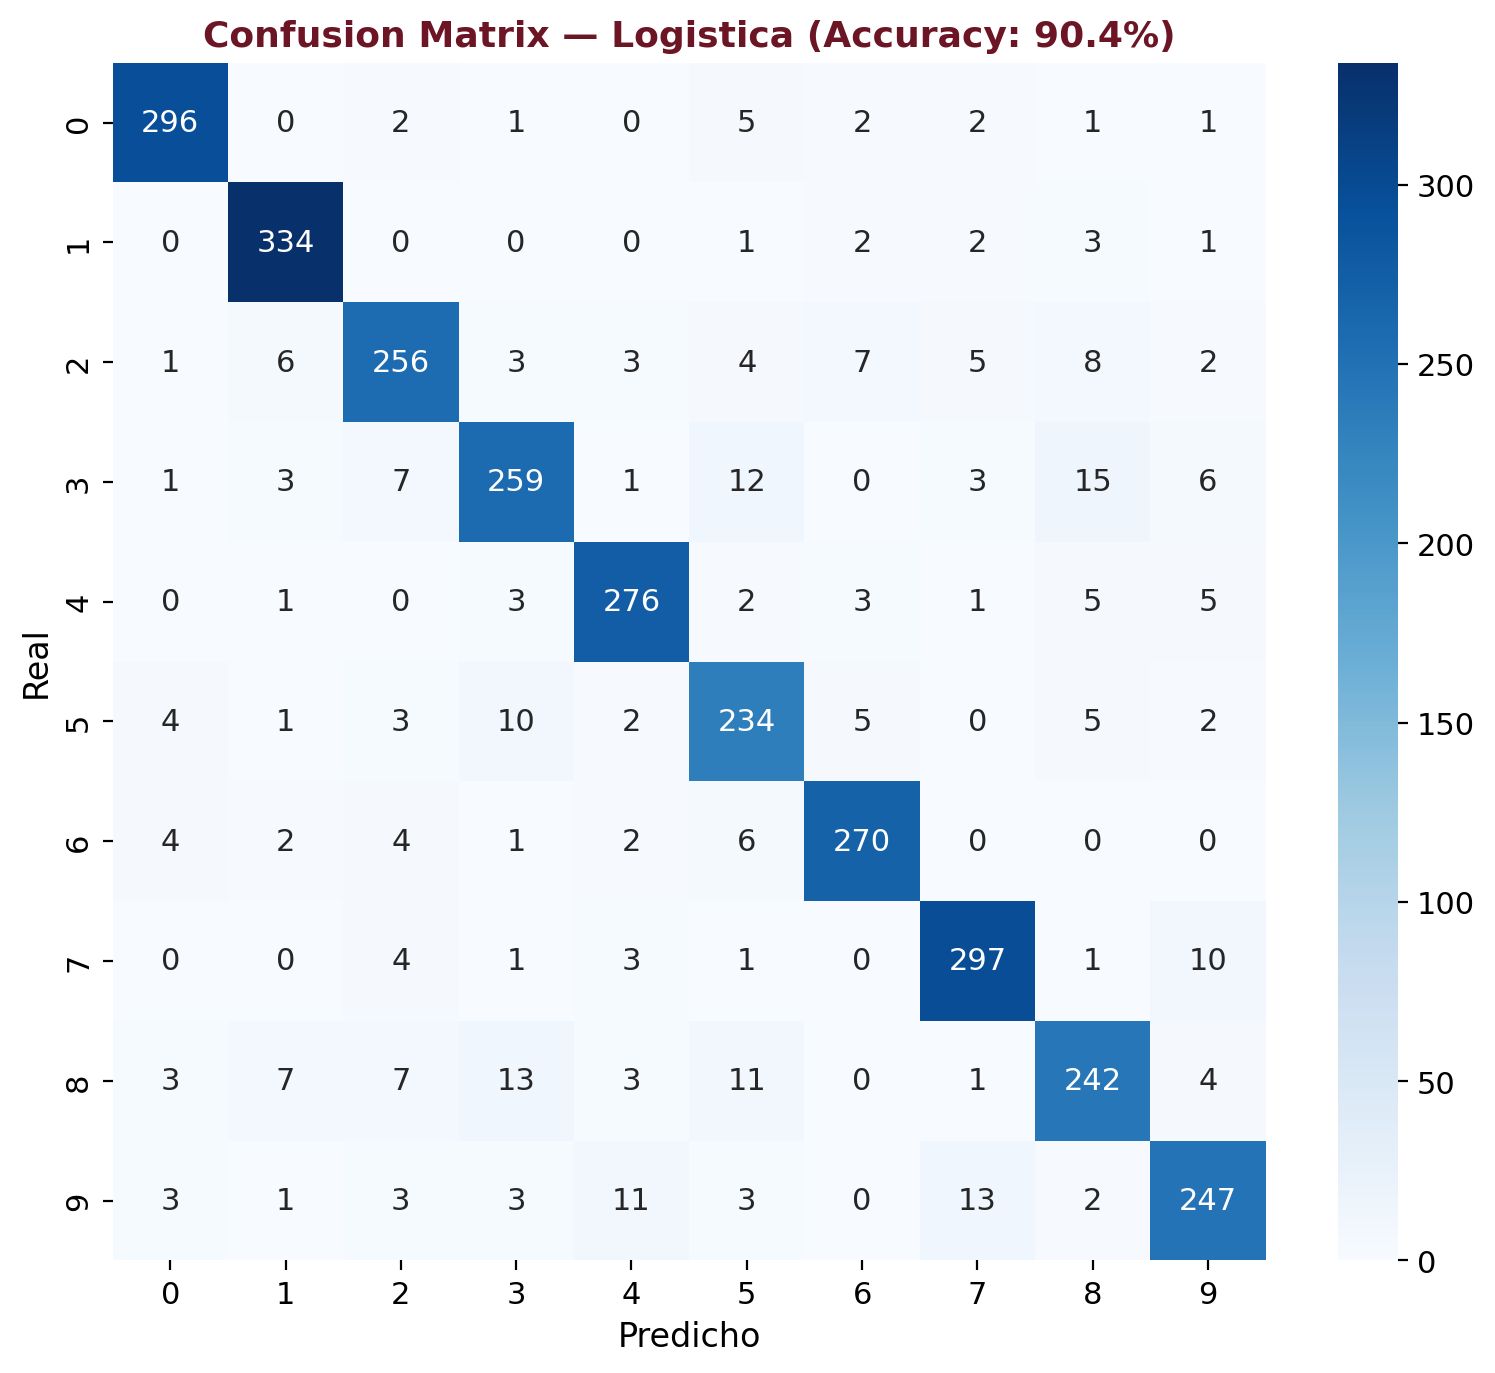
\includegraphics[width=0.55\textwidth]{fig_confusion_lr.png}
  \end{center}

  \vspace{-2pt}
  {\scriptsize\color{textMuted}
    \faLightbulb\hspace{4pt} La diagonal son los aciertos. Fuera de la
    diagonal: errores. Los m\'as comunes: \textbf{3$\leftrightarrow$8},
    \textbf{3$\leftrightarrow$5}, \textbf{9$\leftrightarrow$7},
    \textbf{9$\leftrightarrow$4}. Todos visualmente similares.}
\end{frame}

\begin{frame}[shrink=18]{An\'alisis de Errores: Ver las Im\'agenes Mal Clasificadas}
  \vspace{-4pt}
  \begin{center}
    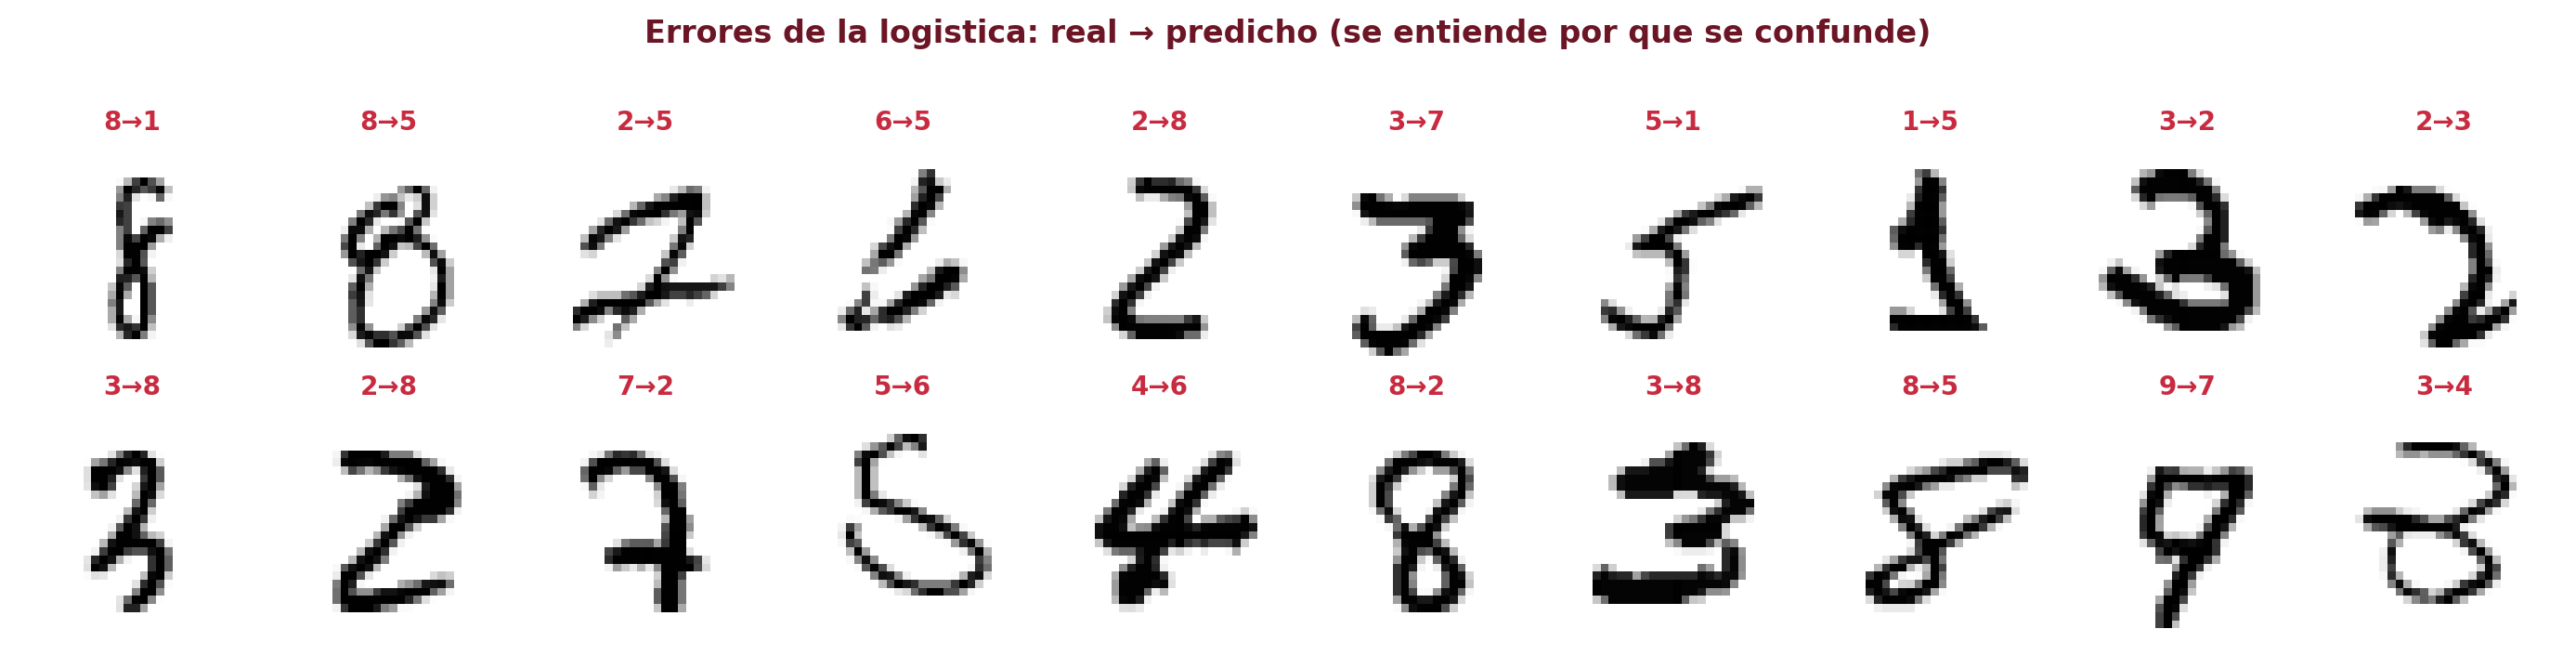
\includegraphics[width=0.9\textwidth]{fig_errores.png}
  \end{center}

  \vspace{-2pt}
  {\scriptsize\color{textMuted}
    \faLightbulb\hspace{4pt} Cada imagen muestra ``real $\to$ predicho''.
    Muchos errores son d\'igitos \textbf{que un humano tambi\'en confundir\'ia}.
    Un ``3'' mal escrito que parece ``8'', un ``9'' que parece ``4''.
    \textbf{El modelo no es tonto --- los datos son ambiguos.}}
\end{frame}

\begin{frame}{Random Forest: M\'as Potencia}
  \vspace{-4pt}
  {\footnotesize\color{arcaDark}\bfseries
    RF no necesita normalizar y captura interacciones entre pixeles:}

  \vspace{6pt}
  {\footnotesize
  \begin{itemize}\setlength{\itemsep}{5pt}
    \item[{\color{codeGreen}\scriptsize\faArrowRight}]
      RF con 200 \'arboles: $\approx$ 94.7\% accuracy (+4.7\% vs log\'istica).
    \item[{\color{codeGreen}\scriptsize\faArrowRight}]
      Mejora en los d\'igitos dif\'iciles (3, 5, 8, 9) porque captura
      \textbf{combinaciones no lineales} entre pixeles.
    \item[{\color{arcaRed}\scriptsize\faArrowRight}]
      Pero sigue confundiendo 3$\leftrightarrow$8 y 9$\leftrightarrow$4
      --- son genuinamente ambiguos.
  \end{itemize}
  }

  \vspace{6pt}
  \begin{tcolorbox}[colback=arcaGray, colframe=arcaRed, boxrule=0.5pt, arc=2pt,
    left=6pt, right=6pt, top=4pt, bottom=4pt]
    {\scriptsize\color{arcaDark}
    \faKey\hspace{4pt}\textbf{Importante:} la mejora de 90\% a 95\% no es
    ``solo 5\%''. Significa que RF comete \textbf{la mitad de errores}
    que log\'istica (de 10\% a 5\%). En 10\,000 cartas son 500 cartas
    menos que se env\'ian mal.}
  \end{tcolorbox}
\end{frame}

\begin{frame}[shrink=18]{Confusion Matrix --- Random Forest}
  \vspace{-4pt}
  \begin{center}
    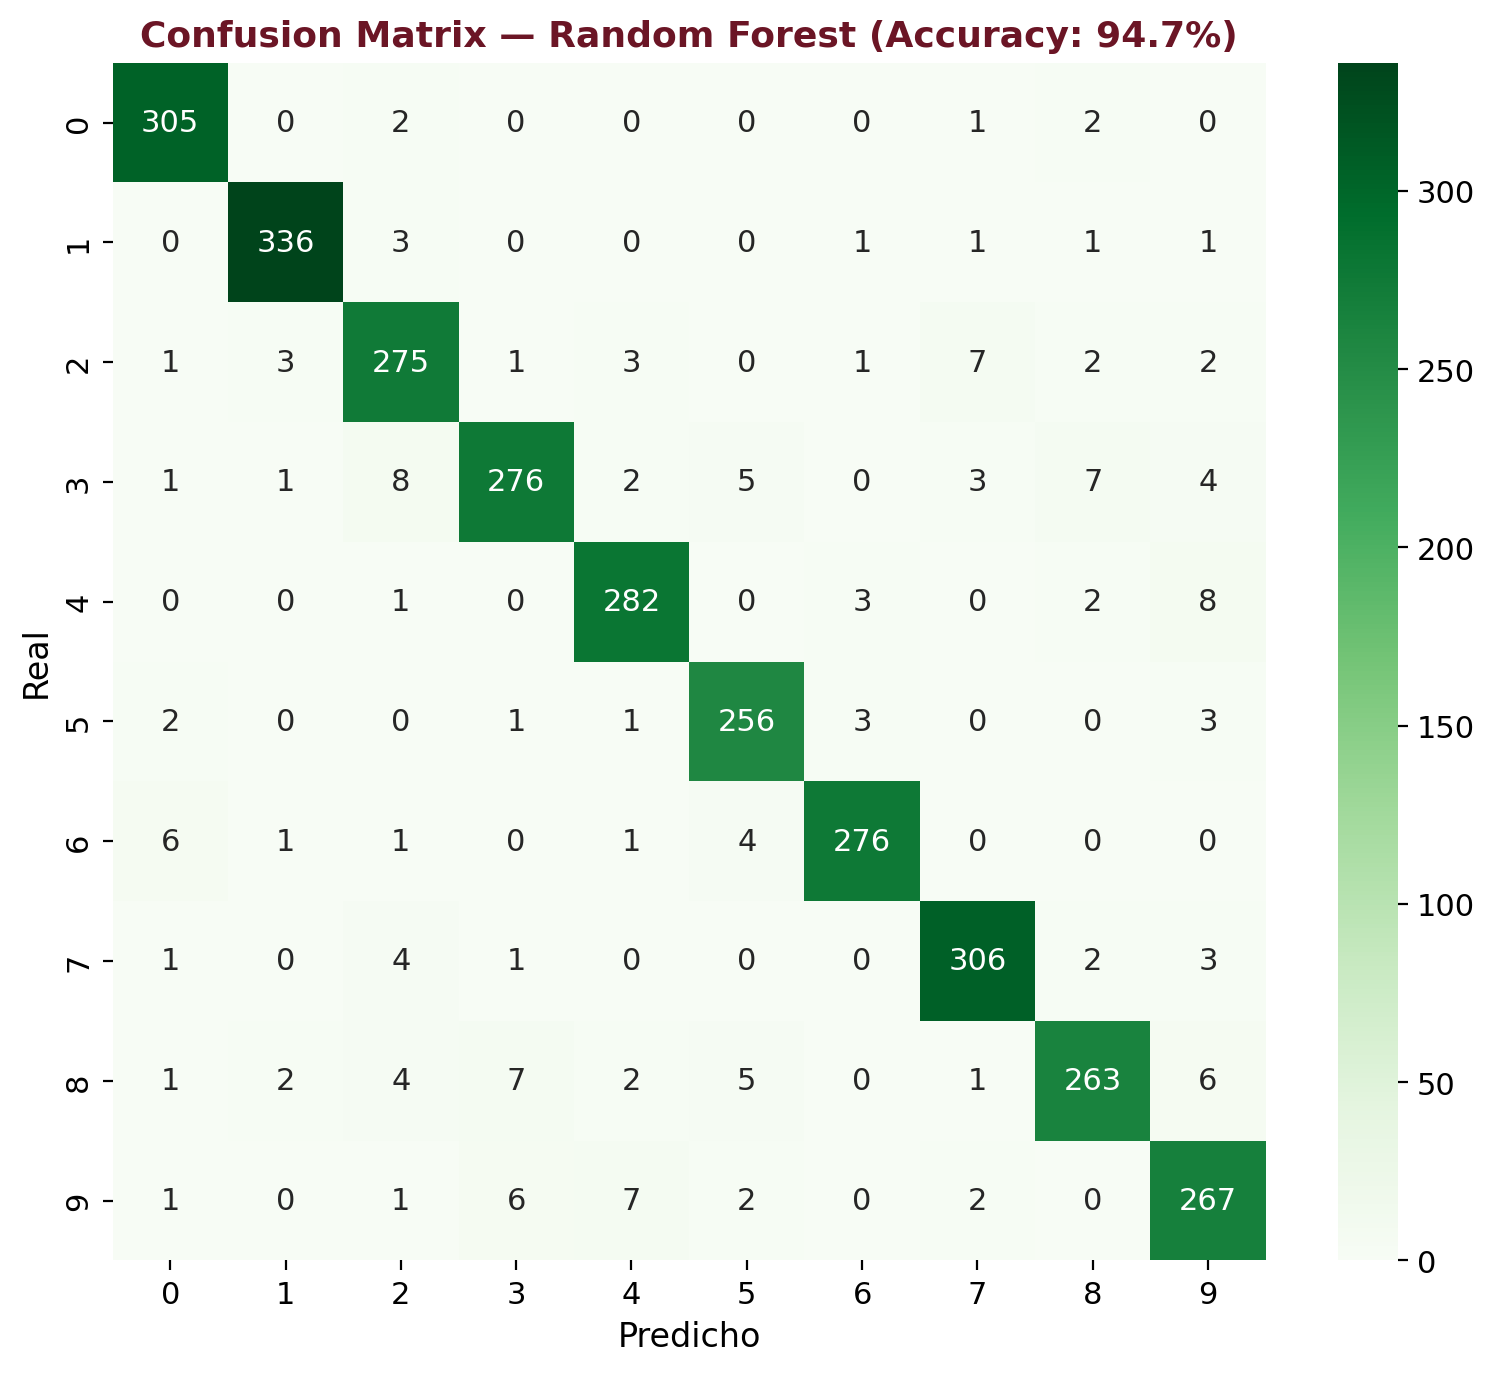
\includegraphics[width=0.55\textwidth]{fig_confusion_rf.png}
  \end{center}

  \vspace{-2pt}
  {\scriptsize\color{textMuted}
    \faLightbulb\hspace{4pt} Menos errores fuera de la diagonal. RF mejora
    especialmente en 5 (confund\'ia con 3) y 8 (confund\'ia con 3 y 5).
    Pero 9$\leftrightarrow$4 sigue siendo dif\'icil.}
\end{frame}

% =============================================================================
%  BLOQUE F: GRADIO
% =============================================================================
\sectionframe{Gradio}{Dibujar un d\'igito y que el modelo lo prediga}

\begin{frame}[fragile,shrink=22]{Demo: Dibujar y Predecir}
  \vspace{-6pt}
  \begin{pyblock}
import gradio as gr
from PIL import Image

def predecir_digito(imagen):
    # Convertir a escala de grises, redimensionar a 28x28
    # Sketchpad devuelve dict en Gradio reciente
    if isinstance(imagen, dict):
        imagen = imagen.get("composite", imagen)
    img = Image.fromarray(imagen).convert("L").resize((28, 28))
    pixels = np.array(img).flatten() / 255.0
    pixels = 1 - pixels   # invertir (Gradio usa fondo blanco)
    pred = rf.predict(pixels.reshape(1, -1) * 255)[0]
    proba = rf.predict_proba(pixels.reshape(1, -1) * 255)[0]
    return {str(i): float(proba[i]) for i in range(10)}

demo = gr.Interface(
    fn=predecir_digito,
    inputs=gr.Sketchpad(type="numpy"),
    outputs=gr.Label(num_top_classes=5),
    title="Dibuja un digito (0-9)")
demo.launch()
  \end{pyblock}

  \vspace{4pt}
  {\scriptsize\color{arcaDark}
    \faMousePointer\hspace{4pt} \texttt{gr.Sketchpad}: el usuario
    \textbf{dibuja} con el mouse. \texttt{gr.Label}: muestra las
    probabilidades de cada clase como barras. El modelo predice en
    tiempo real.}
\end{frame}

% =============================================================================
%  BLOQUE G: FASHION MNIST
% =============================================================================
\sectionframe{Fashion MNIST}{El techo de nuestras herramientas}

\begin{frame}{?`Qu\'e Es Fashion MNIST?}
  \vspace{-4pt}
  {\footnotesize\color{arcaDark}\bfseries
    Creado en 2017 por Zalando (tienda de ropa online) como reemplazo
    de MNIST. Misma estructura, \textbf{mucho m\'as dif\'icil}:}

  \vspace{6pt}
  {\scriptsize
  \begin{tabular}{@{}llp{7cm}@{}}
    \toprule
    \textbf{Propiedad} & \textbf{Valor} & \textbf{Detalle} \\
    \midrule
    Im\'agenes & 70\,000 & Misma cantidad que MNIST. \\
    Tama\~no & 28 $\times$ 28 & Misma resoluci\'on. \\
    Clases & 10 & Camiseta, pantal\'on, su\'eter, vestido, abrigo,
      sandalia, camisa, zapatilla, bolso, bota. \\
    \bottomrule
  \end{tabular}
  }

  \vspace{4pt}
  {\footnotesize
  \begin{itemize}\setlength{\itemsep}{4pt}
    \item[{\color{arcaRed}\scriptsize\faArrowRight}]
      ?`Por qu\'e es m\'as dif\'icil? Una camiseta y una camisa tienen
      la \textbf{misma forma general} --- la diferencia est\'a en
      detalles finos que los pixeles no capturan bien.
    \item[{\color{arcaRed}\scriptsize\faArrowRight}]
      MNIST se resolvi\'o ``demasiado bien'' (99.7\% con CNNs).
      Fashion MNIST sigue siendo desafiante.
  \end{itemize}
  }
\end{frame}

\begin{frame}[shrink=18]{As\'i Se Ve Fashion MNIST}
  \vspace{-4pt}
  \begin{center}
    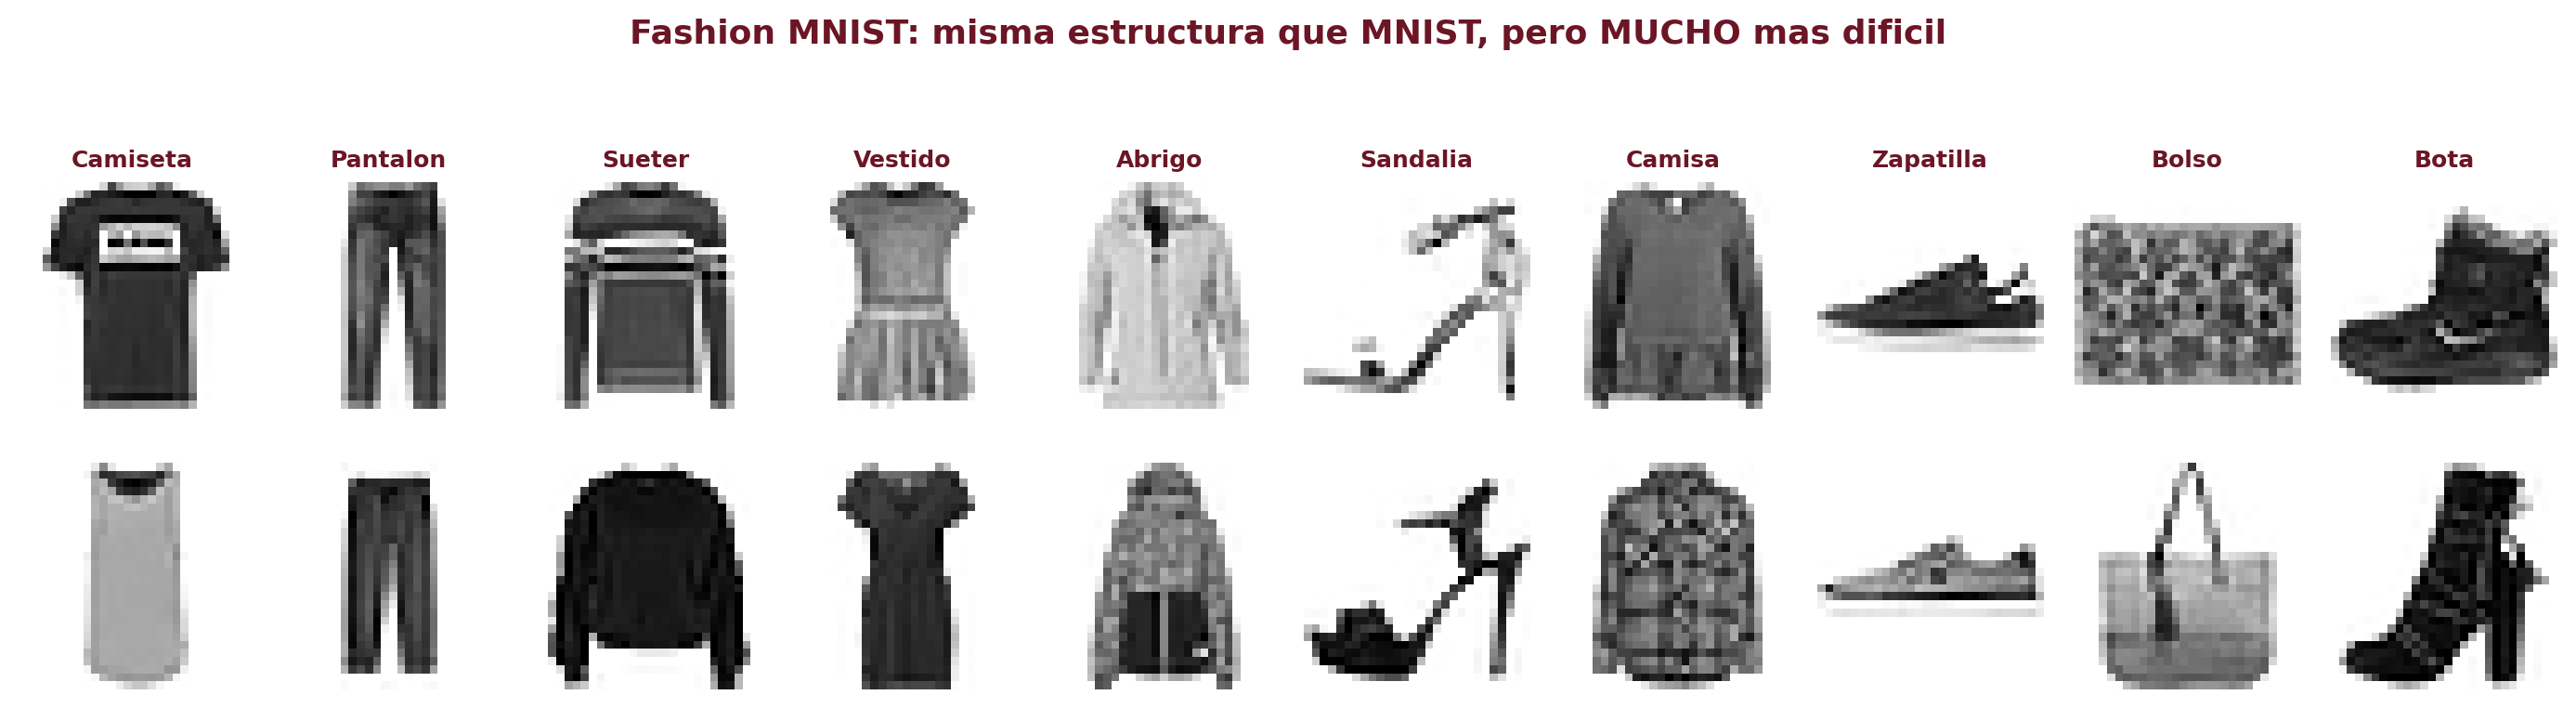
\includegraphics[width=0.88\textwidth]{fig_fashion_samples.png}
  \end{center}

  \vspace{-2pt}
  {\scriptsize\color{textMuted}
    \faLightbulb\hspace{4pt} Misma estructura que MNIST (28$\times$28
    grises) pero el contenido es ropa. Una camiseta y un su\'eter
    se ven muy parecidos en 28$\times$28 pixeles.}
\end{frame}

\begin{frame}[shrink=18]{Comparaci\'on: MNIST vs Fashion MNIST}
  \vspace{-4pt}
  \begin{center}
    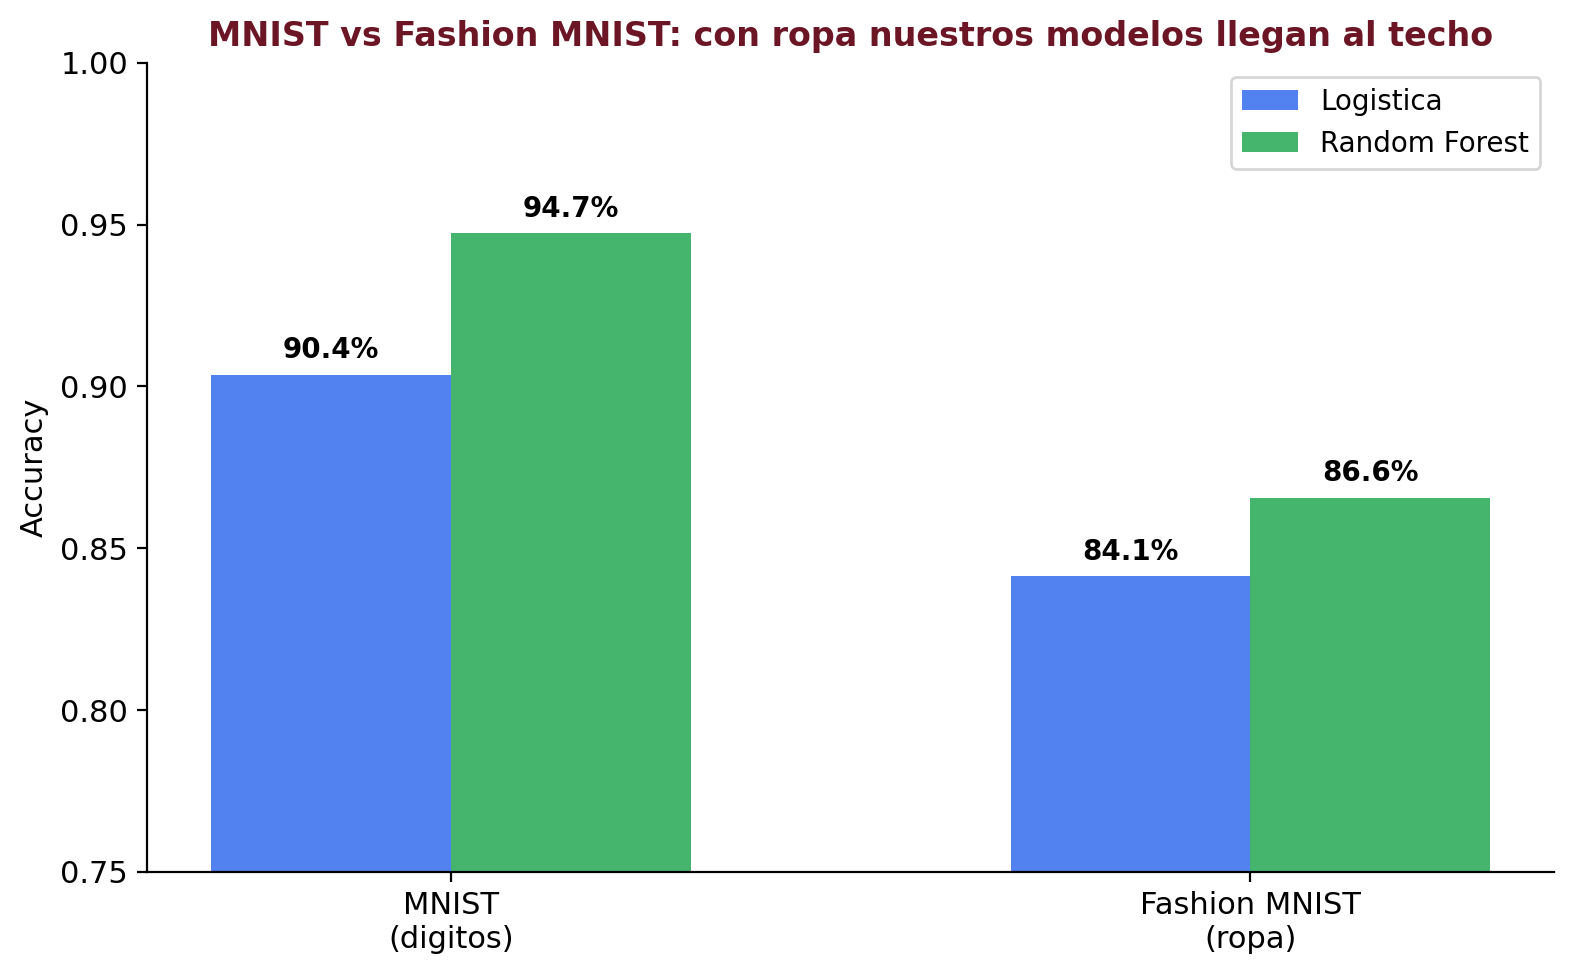
\includegraphics[width=0.7\textwidth]{fig_comparacion_final.png}
  \end{center}

  \vspace{-2pt}
  {\scriptsize\color{textMuted}
    \faLightbulb\hspace{4pt} Los mismos modelos, la misma cantidad de datos.
    Log\'istica baja de 90\% a 84\%. RF baja de 95\% a 87\%.
    \textbf{Con las herramientas que tenemos, este es el techo.}
    Para ir m\'as all\'a se necesitan t\'ecnicas que ``entiendan''
    la estructura espacial de la imagen.}
\end{frame}

% =============================================================================
%  BLOQUE H: QU\'E SIGUE
% =============================================================================
\sectionframe{?`Qu\'e Sigue?}{Una ventana al futuro}

\begin{frame}{El Techo y C\'omo Romperlo}
  \vspace{-4pt}
  {\footnotesize\color{arcaDark}\bfseries
    Nuestros modelos tratan cada pixel como una variable
    \textbf{independiente}. Pero los pixeles tienen
    \textbf{estructura espacial}: los vecinos est\'an relacionados.}

  \vspace{6pt}
  {\footnotesize
  \begin{itemize}\setlength{\itemsep}{5pt}
    \item[{\color{arcaRed}\scriptsize\faArrowRight}]
      \textbf{Log\'istica y RF} ven 784 n\'umeros sueltos. No saben
      que el pixel 100 est\'a \textit{al lado} del pixel 101.
    \item[{\color{arcaRed}\scriptsize\faArrowRight}]
      Un ``3'' girado 10 grados es un vector \textbf{completamente distinto}
      para estos modelos, aunque para nosotros es el mismo d\'igito.
    \item[{\color{codeGreen}\scriptsize\faArrowRight}]
      \textbf{Redes Neuronales Convolucionales (CNN)}: procesan la
      imagen \textit{como imagen} (2D), no como vector. Detectan
      bordes, curvas y formas sin importar la posici\'on.
    \item[{\color{codeGreen}\scriptsize\faArrowRight}]
      CNN en MNIST: 99.7\%. En Fashion MNIST: $\approx$ 93\%.
      En ImageNet (1000 clases, fotos reales): las CNNs superaron
      al humano en 2015.
  \end{itemize}
  }

  \vspace{4pt}
  \begin{tcolorbox}[colback=codeGreen!8, colframe=codeGreen, boxrule=0.5pt, arc=2pt,
    left=6pt, right=6pt, top=4pt, bottom=4pt]
    {\scriptsize\color{arcaDark}
    \faLightbulb\hspace{4pt}\textbf{Lo que aprendieron en este diplomado es la base.}
    Preprocesamiento, EDA, evaluaci\'on con m\'etricas, confusion matrix,
    train/test split, GridSearchCV --- todo eso se reutiliza con CNNs.
    Solo cambia el modelo, no el flujo de trabajo.}
  \end{tcolorbox}
\end{frame}

% =============================================================================
%  CIERRE
% =============================================================================
\sectionframe{Actividad Final}{Crear nuestro propio dataset}

\begin{frame}{Ahora Ustedes Son la Fuente de Datos}
  \vspace{-4pt}
  {\footnotesize\color{arcaDark}\bfseries
    Vamos a crear un dataset de \textbf{vocales escritas a mano}
    entre todos. Cada estudiante dibuja A, E, I, O, U --- 5 veces
    cada una = 25 dibujos por persona.}

  \vspace{6pt}
  {\footnotesize
  \begin{enumerate}\setlength{\itemsep}{4pt}
    \item[{\color{arcaRed}\bfseries 1.}]
      El profesor comparte un \textbf{link p\'ublico de Gradio}.
    \item[{\color{arcaRed}\bfseries 2.}]
      Cada estudiante abre el link en su celular o laptop.
    \item[{\color{arcaRed}\bfseries 3.}]
      Selecciona la vocal, escribe su nombre, dibuja, y env\'ia.
    \item[{\color{arcaRed}\bfseries 4.}]
      Repite 5 veces por vocal = \textbf{25 dibujos} por persona.
    \item[{\color{codeGreen}\bfseries 5.}]
      Todo se guarda autom\'aticamente en un CSV en la m\'aquina
      del profesor.
  \end{enumerate}
  }

  \vspace{4pt}
  \begin{tcolorbox}[colback=codeGreen!8, colframe=codeGreen, boxrule=0.5pt, arc=2pt,
    left=6pt, right=6pt, top=4pt, bottom=4pt]
    {\scriptsize\color{arcaDark}
    \faLightbulb\hspace{4pt}\textbf{El ciclo completo:} ustedes dibujan
    $\to$ recopilamos $\to$ EDA $\to$ PCA + t-SNE $\to$ entrenamos modelos
    $\to$ desplegamos con Gradio. De principio a fin, con datos propios.}
  \end{tcolorbox}
\end{frame}

\begin{frame}{Despu\'es de Recopilar: El Flujo Completo}
  \vspace{-4pt}
  {\footnotesize\color{arcaDark}\bfseries
    Con el CSV de vocales aplicamos todo lo que sabemos:}

  \vspace{6pt}
  {\footnotesize
  \begin{itemize}\setlength{\itemsep}{5pt}
    \item[{\color{arcaRed}\scriptsize\faArrowRight}]
      \textbf{EDA:} visualizar las vocales, promedio por clase,
      varianza por pixel, distribuci\'on de muestras por estudiante.
    \item[{\color{arcaRed}\scriptsize\faArrowRight}]
      \textbf{PCA + t-SNE:} visualizar las 5 vocales en 2D.
      ?`Se separan? ?`Cu\'ales se confunden?
    \item[{\color{arcaRed}\scriptsize\faArrowRight}]
      \textbf{Modelos:} log\'istica + RF. Confusion matrix.
      ?`O se confunde con U? ?`A con E?
    \item[{\color{codeGreen}\scriptsize\faArrowRight}]
      \textbf{Gradio final:} predictor de vocales entrenado con
      \textbf{nuestros propios datos}. Dibujan y el modelo predice.
  \end{itemize}
  }
\end{frame}

% =============================================================================
%  BLOQUE I: DATA AUGMENTATION
% =============================================================================
\sectionframe{Data Augmentation}{M\'as datos sin recopilar m\'as datos}

\begin{frame}{El Problema: Pocas Muestras}
  \vspace{-4pt}
  {\footnotesize\color{arcaDark}\bfseries
    Entre toda la clase recopilamos quiz\'as 200--500 vocales.
    Para entrenar un modelo robusto necesitar\'iamos miles.
    ?`C\'omo conseguimos m\'as datos sin dibujar m\'as?}

  \vspace{8pt}
  {\footnotesize
  \begin{itemize}\setlength{\itemsep}{5pt}
    \item[{\color{arcaRed}\scriptsize\faArrowRight}]
      \textbf{Data Augmentation} = generar datos \textbf{sint\'eticos}
      a partir de los que ya tenemos, aplicando transformaciones que
      \textbf{preservan la clase}.
    \item[{\color{arcaRed}\scriptsize\faArrowRight}]
      Una ``A'' rotada 10 grados sigue siendo una ``A''.
      Una ``A'' desplazada 3 pixeles sigue siendo una ``A''.
    \item[{\color{codeGreen}\scriptsize\faArrowRight}]
      De 1 imagen podemos generar 5--10 variaciones.
      De 200 muestras pasamos a 1000--2000.
  \end{itemize}
  }

  \vspace{6pt}
  \begin{tcolorbox}[colback=arcaGray, colframe=arcaRed, boxrule=0.5pt, arc=2pt,
    left=6pt, right=6pt, top=4pt, bottom=4pt]
    {\scriptsize\color{arcaDark}
    \faKey\hspace{4pt}\textbf{Clave:} la transformaci\'on debe ser
    \textit{realista}. Rotar una ``A'' 10 grados es v\'alido.
    Rotar 180 grados la convierte en otra cosa. Elegir bien las
    transformaciones requiere conocer el dominio.}
  \end{tcolorbox}
\end{frame}

\begin{frame}[shrink=5]{T\'ecnicas de Augmentation M\'as Usadas}
  \vspace{-4pt}
  {\scriptsize
  \begin{tabular}{@{}p{3cm}p{4.5cm}p{5cm}@{}}
    \toprule
    \textbf{T\'ecnica} & \textbf{Qu\'e hace} & \textbf{Cu\'ando usarla} \\
    \midrule
    \textbf{Rotaci\'on} & Gira la imagen $\pm$10--15 grados. & Siempre. La escritura natural var\'ia en \'angulo. \\
    \textbf{Desplazamiento} & Mueve la imagen 2--4 pixeles en cualquier direcci\'on. & Cuando la posici\'on no importa (casi siempre). \\
    \textbf{Zoom} & Agranda o achica 10--20\%. & Cuando el tama\~no var\'ia naturalmente. \\
    \textbf{Ruido gaussiano} & Agrega ruido aleatorio a cada pixel. & Simula variaciones de iluminaci\'on o calidad. \\
    \textbf{Espejo horizontal} & Refleja izquierda-derecha. & \textbf{Cuidado:} en letras NO siempre es v\'alido (una ``b'' espejada es ``d''). \\
    \textbf{Variaci\'on de brillo} & Multiplica los pixeles por un factor. & Simula escr\'aneres o c\'amaras distintas. \\
    \bottomrule
  \end{tabular}
  }

  \vspace{6pt}
  {\scriptsize\color{textMuted}
    \faExclamationTriangle\hspace{4pt}\textbf{Espejo horizontal} no es v\'alido
    para todas las tareas. En vocales: ``A'' espejada sigue siendo ``A'',
    pero en d\'igitos ``6'' espejado podr\'ia parecer ``6'' invertido.
    Conocer el dominio es fundamental.}
\end{frame}

\begin{frame}[shrink=18]{Augmentation --- Visual}
  \vspace{-4pt}
  \begin{center}
    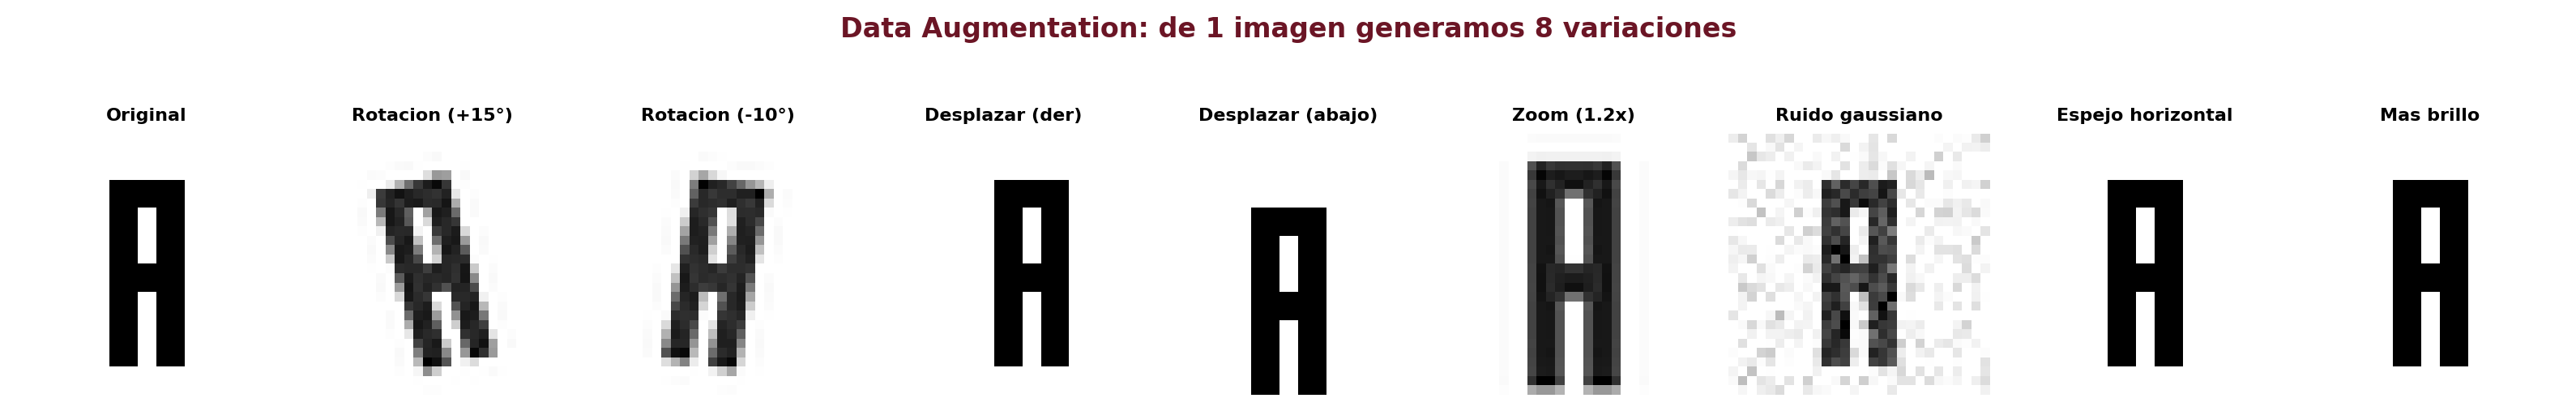
\includegraphics[width=0.95\textwidth]{fig_augmentation.png}
  \end{center}

  \vspace{-2pt}
  {\scriptsize\color{textMuted}
    \faLightbulb\hspace{4pt} De 1 sola imagen generamos 7 variaciones.
    Todas son ``A'' v\'alidas. El modelo ve m\'as diversidad de escritura
    sin necesitar m\'as personas dibujando.}
\end{frame}

\begin{frame}[fragile,shrink=22]{C\'odigo: Augmentation con scipy}
  \vspace{-6pt}
  \begin{pyblock}
from scipy.ndimage import rotate, shift, zoom
import numpy as np

def augmentar(img_28x28, n=5):
    """Genera n variaciones de una imagen 28x28."""
    aumentadas = []
    for _ in range(n):
        aug = img_28x28.copy().astype(float)
        # Rotacion aleatoria
        angulo = np.random.uniform(-15, 15)
        aug = rotate(aug, angulo, reshape=False, mode="constant")
        # Desplazamiento aleatorio
        dx, dy = np.random.randint(-3, 4, 2)
        aug = shift(aug, [dy, dx], mode="constant")
        # Ruido
        aug += np.random.normal(0, 10, aug.shape)
        aumentadas.append(aug.clip(0, 255).astype(np.uint8))
    return aumentadas
  \end{pyblock}

  \vspace{4pt}
  {\scriptsize\color{arcaDark}
    \faKey\hspace{4pt} Cada llamada genera \texttt{n} im\'agenes nuevas
    con rotaci\'on, desplazamiento y ruido aleatorios. De 200 muestras
    con \texttt{n=5} obtenemos 1200 (200 originales + 1000 sint\'eticas).}
\end{frame}

\begin{frame}{?`Cu\'anto Mejora? --- Depende}
  \vspace{-4pt}
  {\footnotesize\color{arcaDark}\bfseries
    Data augmentation no es magia. Funciona bien cuando:}

  \vspace{6pt}
  {\footnotesize
  \begin{itemize}\setlength{\itemsep}{5pt}
    \item[{\color{codeGreen}\scriptsize\faCheckCircle}]
      \textbf{Pocos datos} (menos de 500 por clase). M\'as impacto.
    \item[{\color{codeGreen}\scriptsize\faCheckCircle}]
      \textbf{Transformaciones realistas}: las variaciones se parecen
      a lo que ocurrir\'ia en la realidad.
    \item[{\color{arcaRed}\scriptsize\faTimesCircle}]
      \textbf{Muchos datos}: si ya tienes 10\,000 por clase, el impacto
      es marginal.
    \item[{\color{arcaRed}\scriptsize\faTimesCircle}]
      \textbf{Transformaciones no realistas}: rotar una foto de un auto
      180 grados no es un auto real.
  \end{itemize}
  }

  \vspace{6pt}
  \begin{tcolorbox}[colback=codeGreen!8, colframe=codeGreen, boxrule=0.5pt, arc=2pt,
    left=6pt, right=6pt, top=4pt, bottom=4pt]
    {\scriptsize\color{arcaDark}
    \faLightbulb\hspace{4pt}\textbf{En la industria:} data augmentation
    es est\'andar en visi\'on por computadora. Todas las CNN modernas
    lo usan durante el entrenamiento. Es gratis y casi siempre ayuda.}
  \end{tcolorbox}
\end{frame}

% =============================================================================
%  CIERRE
% =============================================================================
\sectionframe{Cierre}{Lo que aprendimos hoy}

\begin{frame}[shrink=10]{Resumen}
  \vspace{-4pt}
  \begin{columns}[T]
    \begin{column}{0.48\textwidth}
      {\footnotesize\bfseries\color{arcaDark} Im\'agenes como datos:}
      \vspace{4pt}

      {\footnotesize
      \begin{itemize}\setlength{\itemsep}{3pt}
        \item[{\color{codeGreen}\faCheckCircle}]
          Imagen = matriz de n\'umeros (pixeles).
        \item[{\color{codeGreen}\faCheckCircle}]
          Para ML: aplanar a vector (28$\times$28 $\to$ 784).
        \item[{\color{codeGreen}\faCheckCircle}]
          EDA: promedios, varianza, distribuciones.
        \item[{\color{codeGreen}\faCheckCircle}]
          Normalizar: dividir entre 255.
      \end{itemize}
      }

      \vspace{4pt}
      {\footnotesize\bfseries\color{codeBlue} Modelos:}
      \vspace{4pt}

      {\footnotesize
      \begin{itemize}\setlength{\itemsep}{3pt}
        \item[{\color{codeGreen}\faCheckCircle}]
          Log\'istica: $\approx$ 90\% (baseline s\'olida).
        \item[{\color{codeGreen}\faCheckCircle}]
          Random Forest: $\approx$ 95\% (mejor en d\'igitos dif\'iciles).
        \item[{\color{codeGreen}\faCheckCircle}]
          An\'alisis de errores: ver las im\'agenes mal clasificadas.
      \end{itemize}
      }
    \end{column}

    \begin{column}{0.48\textwidth}
      {\footnotesize\bfseries\color{arcaRed} El techo:}
      \vspace{4pt}

      {\footnotesize
      \begin{itemize}\setlength{\itemsep}{3pt}
        \item[{\color{codeGreen}\faCheckCircle}]
          Fashion MNIST: 84--87\% con nuestras herramientas.
        \item[{\color{codeGreen}\faCheckCircle}]
          El problema: tratamos pixeles como independientes.
        \item[{\color{codeGreen}\faCheckCircle}]
          CNNs rompen ese techo (99\%+ en MNIST).
      \end{itemize}
      }

      \vspace{4pt}
      {\footnotesize\bfseries\color{codePurple} Gradio:}
      \vspace{4pt}

      {\footnotesize
      \begin{itemize}\setlength{\itemsep}{3pt}
        \item[{\color{codeGreen}\faCheckCircle}]
          \texttt{gr.Sketchpad}: dibujar con el mouse.
        \item[{\color{codeGreen}\faCheckCircle}]
          \texttt{gr.Label}: mostrar probabilidades.
        \item[{\color{codeGreen}\faCheckCircle}]
          El modelo predice en tiempo real.
      \end{itemize}
      }
    \end{column}
  \end{columns}
\end{frame}

% ── QR ENCUESTA ──────────────────────────────────────────────────────────────
{
\setbeamertemplate{headline}{}
\setbeamertemplate{footline}{}
\begin{frame}[plain, noframenumbering]
  \begin{tikzpicture}[remember picture, overlay]
    \fill[arcaDark] (current page.south west) rectangle (current page.north east);
  \end{tikzpicture}
  \vspace{1cm}
  \begin{center}
    {\Huge\bfseries\color{white} ?`C\'omo estuvo la clase?\par}
    \vspace{0.6cm}
    
\includegraphics[width=4cm]{qr_encuesta.jpg}
    \vspace{0.4cm}

    {\large\color{white!80} Escanea el QR para dejarnos tu opini\'on.\par}
  \end{center}
\end{frame}
}

\end{document}
